\documentclass[12pt,a4paper,oneside,onecolumn]{article}

\usepackage[spanish,es-noshorthands]{babel}
\usepackage{epsfig}
\usepackage[latin1]{inputenc}
\usepackage{amsmath}
\usepackage{amsfonts}
\usepackage{amssymb}
%\usepackage{mathabx}  Compila pero borra el pdf?
\usepackage{array}
\usepackage[left=1.8cm, right=1.8cm, top=2.50cm, bottom=2.5cm]{geometry}
\usepackage{hyperref}
\usepackage{color}
\usepackage{fancyhdr}
\usepackage{listings}
\usepackage{xcolor}

\pagestyle{fancy}

\fancyhead{}
\fancyfoot{}

\setlength{\headsep}{0.4cm}
\setlength{\footskip}{1.6pt}
\setlength{\parindent}{0pt}
\setlength{\extrarowheight}{1.5pt}


\lhead{Proyectos II}
\rhead{Javier Orti}
\renewcommand*\headrulewidth{0.4 pt}
\lfoot{\vspace{0.45cm}SQL injection}
\cfoot{\vspace{0.01cm}\rule{\linewidth}{0.4pt}}
\rfoot{\vspace{0.45cm} P\'ag. \thepage}

\renewcommand{\labelitemi}{$\bullet$}
\renewcommand{\labelenumi}{\theenumi)}
\renewcommand\spanishtablename{Tabla}

\decimalpoint

\headheight 16.7pt 
\textheight 715pt 

\parskip 8pt  

\hypersetup{
	colorlinks=true,
	linkcolor=blue,
	filecolor=magenta,      
	urlcolor=cyan,
}

% Python code settings
\definecolor{codegreen}{rgb}{0,0.6,0}
\definecolor{codegray}{rgb}{0.5,0.5,0.5}
\definecolor{codepurple}{rgb}{0.58,0,0.82}
\definecolor{backcolour}{rgb}{0.95,0.95,0.92}

\lstdefinestyle{mystyle}{
	backgroundcolor=\color{backcolour},   
	commentstyle=\color{codegreen},
	keywordstyle=\color{magenta},
	numberstyle=\tiny\color{codegray},
	stringstyle=\color{codepurple},
	basicstyle=\ttfamily\footnotesize,
	breakatwhitespace=false,         
	breaklines=true,                 
	captionpos=b,                    
	keepspaces=true,                 
	numbers=left,                    
	numbersep=5pt,                  
	showspaces=false,                
	showstringspaces=false,
	showtabs=false,                  
	tabsize=2
}

\lstset{style=mystyle}

\usepackage[shortlabels]{enumitem}
\usepackage{cancel}

\begin{document} 
    \section{}
    Una SQLi es un vector de ataque t\'ipico en la red que consiste en lanzar comandos maliciosos 'enmascarados' como parte de una query a una base de datos relacional, para extraer datos o modificar datos inaccesibles, incluso con la posibilidad de borrar toda la base de datos (el cl\'asico DROP DATABASE).
    \newline
    Los tipos son:
    \begin{enumerate}[a)]
        \item
        \underline{In-band SQLi:} El atacante utiliza el mismo canal para lanzar su ataque y obtener los resultados. Este tiene dos subvariantes principales. Primero SQLi basado en errores, para que la base de datos devuelva mensajes de error y el hacker pueda obtener datos principalmente de la estructura de la DB. Segundo el Union, en el que se aprovecha del operador UNION para fusionar varios comandos, por ejemplo de selecci\'on en una sola HTTP response.
        \item
        \underline{Out-of-band SQLi:} El 'opuesto' al anterior, que solo podrá ser utilizado si la estructura atacada tiene una distribuci\'on concreta. Como bien dice el nombre, el atacante no puede recibir la informaci\'on por el mismo canal por el que lanza las queries.
        \item
        \underline{Inferential (Blind) SQLi:} Son aquellos ataques en los que el agresor no recibe respuesta directa de la DB como en los ejemplos anteriores, por los que estos se basan en las respuestas y patrones de comportamientos que de el servidor al cliente, por lo que suelen ser los ataques m\'as complejos de realizar. Una forma de clasificarlos es en booleanos y time-based. Los booleanos tratan de lanzar consultas verdaderas o falsas, que por tanto generaran una HTTP response diferente. Por \'ultimo los time-based, que como dice el nombre, se basan en el tiempo de respuesta del servidor, ya que seg\'un la duraci\'on total de la petici\'on se puede llegar a deducir si la query que se lanz\'o al server devolvi\'o true o false.
    \end{enumerate}
    
    \begin{figure}[!h]
		\centering
		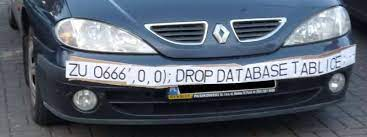
\includegraphics[scale=1.2]{SQLi.jpg}
		\caption{}
		\label{fig:1}
	\end{figure}
	\newpage
	\section{}
	
	\begin{enumerate}
	\item 
	Entender cuando interactua el server con la DB y hacer una lista de campos de inputs que podr\'ian usarse en la consulta.
	\item 
	Penetrar la consulta con comillas simples, dobles, backticks o puntos y comas, prestando atenci\'on a cualquier error o malfuncionamiento de la aplicaci\'on.
	\item 
	Ah\'i dependemos de que el server lance mensajes de error al usuario. En caso afirmativo podriamos encontrar un input, por ejemplo el nombre de una tabla \emph{table\_name}.
	\item A partir de a\'i empieza lo gordo ya que podemos acceder a las columnas.
	\end{enumerate}
	
	\section{}
	\begin{enumerate}
	\item 
	Uso de queries preparadas y parametrizadas, as\'i el atacate no puede escribir comandos completos(en principio).
	\item
	Funciones almacenadas, misma l\'ogica que el anterior, pero son procedimientos ya almacenados en la propia DB.
	\item
	validaci\'on de inputs con una lista de entrada. En el servidor se crea una lista en la que solo se permite la ejecuci\'on si los par\'ametros de la petici\'on se encuentran en una lista creada por el defensor.
	
	\end{enumerate}
	
	\section{}
	Hay muchos truquillos para esquivar los flitros, entre ellos se encuentran:
	\begin{enumerate}
	\item 
	Espacios en blanco, tabulaciones... Ya que no afectan a la query original y nos permiten a\~nadir codigo malicioso.
	\item
	Bytes nulos. Si por ejemplo se est\'an bloqueando los ap\'ostrofes, la siguiente inyecci\'on podr\'ia ayudar: \emph{\%00' or 1=1- -}
	\item
	Codificaci\'on de URL. Para poder enviar queries y par\'ametros a traves del protocolo HTTP.
	\item
	Codificaci\'on hexadecimal. Convirtiendo los caracteres ASCII en su equivalente hexadecimal
	\item
	Concatenando strings. Un ejemplo podr\'ia ser: \emph{CONCAT('SEL', 'ECT')}
	\item 
	Usando comentarios se puede evadir filtros b\'asicos que tenga el servidor ya que como en cualquier lenguaje, se pueden usar tantos comentarios como se quieran.
	\end{enumerate}
	
	\section{}
	Por supuesto que s\'i, ya que para empezar servicios como mysql permiten ejecutar shell commands desde dentro. Un ejemplo para ejecutar el comando whoami y obtener informaci\'on del usuario del OS en la DVWA(low security) ser\'ia primero entender mejor como funciona la base de datos, por
	
\end{document}